\documentclass[11pt]{article}
\usepackage[sc]{mathpazo}
\usepackage{amsmath,pifont}
\usepackage{fullpage}
\usepackage[authoryear,sectionbib,sort]{natbib}
\linespread{1.7}
\usepackage[utf8]{inputenc}
\usepackage{lineno}

\usepackage{graphicx} 
\usepackage{tabularx,setspace}

\title{Density-dependent selection and the limits of relative fitness}
\author{Jason Bertram $^{1,\ast}$ \\ 
Joanna Masel $^{1}$}

\date{}

\begin{document}

\maketitle

\noindent{}1. Department of Ecology and Evolutionary Biology, University of Arizona, Tucson, AZ 85721.

\noindent{}$\ast$ Corresponding author; e-mail: jbertram@email.arizona.edu.


\bigskip

%\textit{Manuscript elements}: 

\bigskip

\textit{Keywords}: Lottery model, competitive Lotka-Volterra, $r$/$K$-selection, interference competition, $R^*$ theory, eco-evo.

\bigskip


\linenumbers{}
\modulolinenumbers[1]

\newpage{}

\section*{Abstract}

Evolutionary biologists frequently describe selection using relative fitness, and relative fitness models are foundational in population genetics. Yet the population ecological basis of relative fitness is poorly understood, and the classical ecology literature on selection in crowded populations seems to be incompatible with widely-used relative fitness models such as the Wright-Fisher. Here we develop a generalization of the Wright-Fisher model in which density depends dynamically on the demographic rates of the types present. We then explore the population ecology of relative fitness using this model as a reference point. Although density-dependent selection can cause relative fitness to break down, relative fitness models are fairly robust in populations close to demographic equilbrium. In particular, relative fitness only breaks down if selection is strong and density-dependent, and density is also selection-dependent. Our generalized Wright-Fisher model clearly distinguishes between three demographic parameters, each of whose behavior is, on its own, correctly described by relative fitness models. In contrast, the classical literature on density-dependent selection confounds them. We argue that selection-independent density is ecologically plausible for many species given the prevalence of reproductive excesses, an important aspect of selection omitted in many ecological models. Our model also offers a natural alternative to relative fitness when the latter is untenable, as is likely the case far from demographic equilibrium. 

\newpage{}


\section*{Introduction}

There are a variety of different measures of fitness. Some widely used examples in evolutionary ecology are expected lifetime reproductive ratio $R_0$, intrinsic population growth rate $r$, saturation population density (often labeled ``$K$'') \citep{benton_2000}, and invasion fitness \citep{metz_1992}. In addition, ``relative fitness'' is the standard in much of evolutionary biology, particularly evolutionary genetics, where attention is generally restricted to relative genotypic proportions \cite[pp. 468]{barton_2007}. The variety of fitness measures is not problematic in itself, because different measures  may be more useful in different circumstances. But it should be clear how the measure being used is connected to the processes of birth and death which govern population biology \citep{metcalf_2007,doebeli_2017}. While such a connection is fairly clear for absolute fitness measures like $r$, relative fitness seems largely divorced from population biology. It has even been proposed that relative fitness be justified from more abstract measure-theoretical arguments, abandoning population biology altogether \citep{wagner_2010}.

In uncrowded populations, relative fitness simply represents differences in intrinsic population growth rate. In discrete time, the change in frequency of type $i$ is $\Delta p_i=\left(\frac{W_i}{\overline{W}}-1\right) p_i$, where $W_i$ is the intrinsic absolute growth factor of type $i$, and $\overline{W}=\sum_i W_i p_i$ is the population mean $W$. Here we can rescale $W$ however we please and replace it with ``relative fitness'' $w$ without affecting the ratio $\frac{W_i}{\overline{W}}=\frac{w_i}{\overline{w}}$. In continuous time, the canonical selection equation is $\frac{d p_i}{dt}=(r_i-\overline{r}) p_i$, where $W$ is replaced by the intrinsic exponential growth rate $r$ \citep[pp. 26]{crow_1970}. If there are two types present, a wildtype and a mutant for instance, then the continuous time canonical selection equation can be written as
\begin{equation}
\frac{d p_i}{dt}=s p_i(1-p_i), \label{eq:canonical}
\end{equation}
where the constant selection coefficient $s$ is the difference in $r$ between types. The corresponding adaptive sweeps follow a logistic curve. 

The difficulty with Eq.~\eqref{eq:canonical} arises in crowded populations. Since crowded and uncrowded conditions are so different, $s$ will often depend on density. Eq.~\eqref{eq:canonical} is then no longer a complete description of selection --- we would also need to specify a model for density. Note that frequency-dependent selection does not raise similar problems; Eq.~\eqref{eq:canonical} is still a complete description of selection even if its behavior is more complicated compared to the constant-$s$ case. Standard population genetics evades the issue of density-dependent selection by simply assuming that total population density $N$ has reached its equilibrium value, which is assumed to be a fixed constant. The selection coefficient $s$ now parameterizes the rate at which selection changes relative frequencies, but no longer corresponds to differences in intrinsic growth rates $r$. 

Counter to the assumption of constant $N$, MacArthur famously showed that when population growth is density-regulated, selection in crowded populations is intimately connected to the ability to keep growing at higher densities than other types can tolerate \citep{macarthur_1967}. The classic example is the logistic model, where the type with the greatest saturation population density ``$K$'' excludes the others (Fig.~\ref{fig:Ksel}a). Similarly, the ``$R^*$ rule'', a central tenet of resource competition theory, states that when growth is limited by a single homogeneous consumable resource, the type able to deplete the resource to the lowest equilibrium density $R^*$ excludes the others \citep{grover_1997}. Differences in $R^*$ will often entail differences in saturation density. The Lotka-Volterra competition model also couples selection in crowded populations to changes in $N$ except in a few special cases (we return to this in section ``$K$-selection versus relative fitness''). In these examples, both $N$ and $s$ change during, and as a result of, adaptive sweeps. It would therefore seem that the ubiquitous constant-$N$, relative fitness description of selection is incompatible with a huge class of population ecological processes driving selection (Fig.~\ref{fig:Ksel}b).

\begin{figure}
\centering
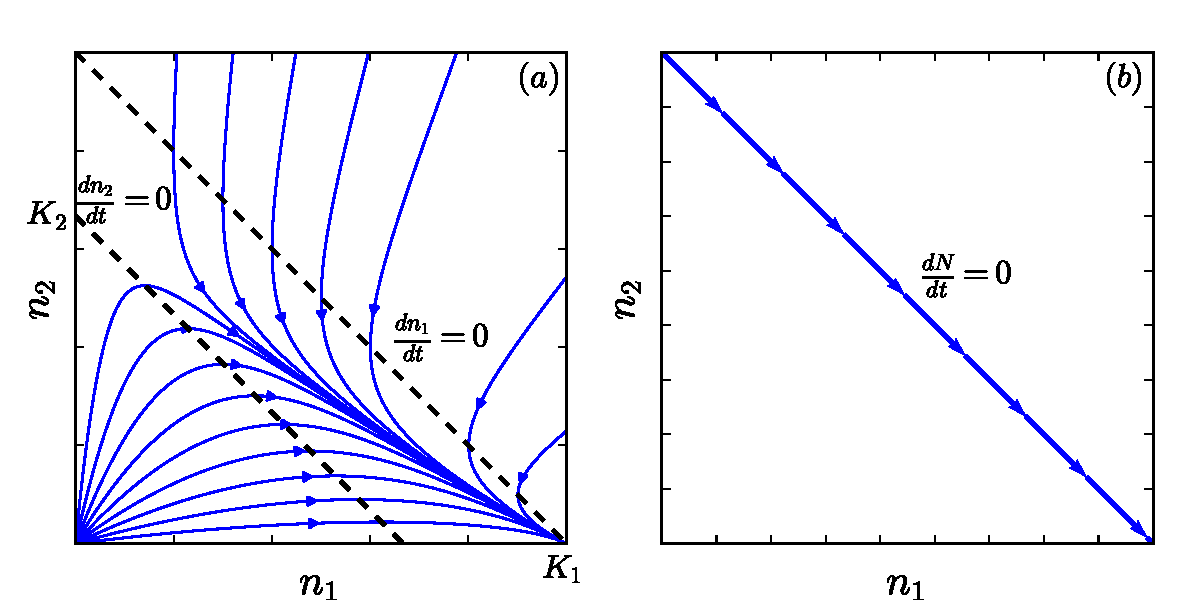
\includegraphics[scale=0.8]{Kplot.pdf}
\caption{\label{fig:Ksel} Selection in crowded environments shown as a phase diagram for the densities of two types $n_1$ and $n_2$. (a) The logistic model $\frac{dn_1}{dt}=r_1(1-\frac{n_1+n_2}{K_1})n_1$ and $\frac{dn_2}{dt}=r_2(1-\frac{n_1+n_2}{K_2})n_1$ with $r_1=r_2$ and $K_1>K_2$. (b) The constant-$N$, relative fitness description of selection.}
\end{figure}

The relative fitness description has been justified in broadly two different ways for crowded populations (we do not discuss Wagner's [\citeyear{wagner_2010}] measure-theoretical justification, which is explicitly independent of population biology and thus falls outside of our scope). The first is to assume that selection is independent of density but still allow density to be affected by selection \citep[pp. 468]{barton_2007} \citep{prout_1980}. While this  allows us to relax the assumption of constant $N$, it does not address the problem that $s$  can, in reality, depend on density. In the examples from the previous paragraph, selection is density-dependent; indeed, the type-specific responses to density are at the center of MacArthur's argument and the density-dependent selection literature that grew out of it \citep{roughgarden_1979}. 

Second, constant $N$ and $s$ can both be seen as a short-term linear approximation \cite[pp. 277]{ewens_2004}. That is, within a sufficiently short time frame, $N$ and $s$ can be treated as constant. Provided that selection is sufficiently weak and stable over time, this ``short-term''  assumption is not a major restriction. Yet it is increasingly recognized that selection is not always weak, that it can fluctuate considerably over time, and that $N$ can vary by orders of magnitude over a few generations as a routine feature of a population's ecology \citep{messer_2016}. These are not rare exceptions, but occur widely in nature and the lab, including in wild \textit{Drosophila} \citep{bergland_14}. Nevertheless, relative fitness models are the foundation for much of the population genetic literature, and are still widely used without considering the ``short-term'' restriction or the lack of integration with population ecology \citep{mallet_2012}. Thus, it is important to understand the population ecological basis of relative fitness models, both to gain insight into their domain of applicability, and as part of the broader challenge of synthesizing ecology and evolution.

Another issue with the constant-$N$ relative fitness description of selection is that it precludes consideration of longer-term aspects of the interplay between evolution and ecology such as population extinction. [will make this sound less dismissive] Adaptive dynamics currently provides a powerful framework for addressing the complex feedbacks between evolutionary change and population density, including but not limited to extinction \citep{diekmann_2004}. However, the focus of adaptive dynamics is trait evolution rather than the underlying genetics, and in particular, selective sweeps are typically subsumed into effectively-instantaneous ``trait substitutions''. We emphasize that our focus here is the description of the time-dependent process by which selection changes allele frequencies, which is particularly critical for making sense of evolution at the genetic level for which we now have abundant data.

Here we analyze the population ecology of relative fitness using a novel model of density-dependent population growth based on territorial contests. Rather attempting to make sense of relative fitness in existing standard models of population growth mentioned above (e.g. \citep{kimura1969natural,mallet_2012}), we instead do the reverse, and attempt to make population ecological sense of the widely-used Wright-Fisher, constant-$N$, relative fitness model. Our starting point is the classic lottery model of territorial contest \citep{sale_77,chesson_1981}. Like the Wright-Fisher model, the classic lottery assumes a saturated population with constant $N$, and fitness involves a product of fertility and juvenile viability \citep[pp. 185]{crow_1970}. Unlike the Wright-Fisher model, generations can overlap in the lottery model. We generalize the lottery model to allow population density to vary, creating a density-dependent generalization of the Wright-Fisher model with overlapping generations. 

We show that when this model reaches a demographic steady-state, the constant-$N$, relative fitness picture emerges. Futhermore, we show that our model is entirely consistent with MacArthur's analysis of selection in crowded populations. In particular, we emphasize that MacArthur's argument does not justify the widespread intuition that selection in crowded environments is necessarily connected to achieving greater densities. This intuition is largely an artifact of the models historically used in the density-dependent selection literature, which ignore the existence of relative contests. 

Our first task is to analytically extend the classic lottery model to correctly account for low density behavior (sections ). We then...[BLAH]

 
\section*{Model}\label{sec:model}

\subsection*{Model assumptions and definitions} 

We assume that reproductively mature individuals (``adults'') each require their own territory to survive and reproduce (Fig.~\ref{fig:lottery}). All territories are identical, and the total number of territories is $T$. Time advances in discrete iterations, each representing the time from birth to reproductive maturity. In a given iteration the number of adults of the $i$'th type will be denoted $n_i$, the total number of adults by $N=\sum_i n_i$, and the number of unoccupied territories by $U=T-N$. 

We assume that the $n_i$ are large enough that stochastic fluctuations in the $n_i$ (``drift'') can be ignored. In particular, we do not evaluate the initial stochastic behaviour of mutant lineages while they are at low abundance. We derive equations for the expected change in the $n_i$ over time, leaving the evaluation of drift for future work.  

%When considering new mutations, we therefore restrict our attention to the earliest (lowest $n_i$) deterministic behavior of mutant lineages (the transition to deterministic growth occurs at an abundance $n_i$ of order equal to their inverse expected absolute growth rate; \citealt{uecker_2011}).

\begin{figure}
\centering
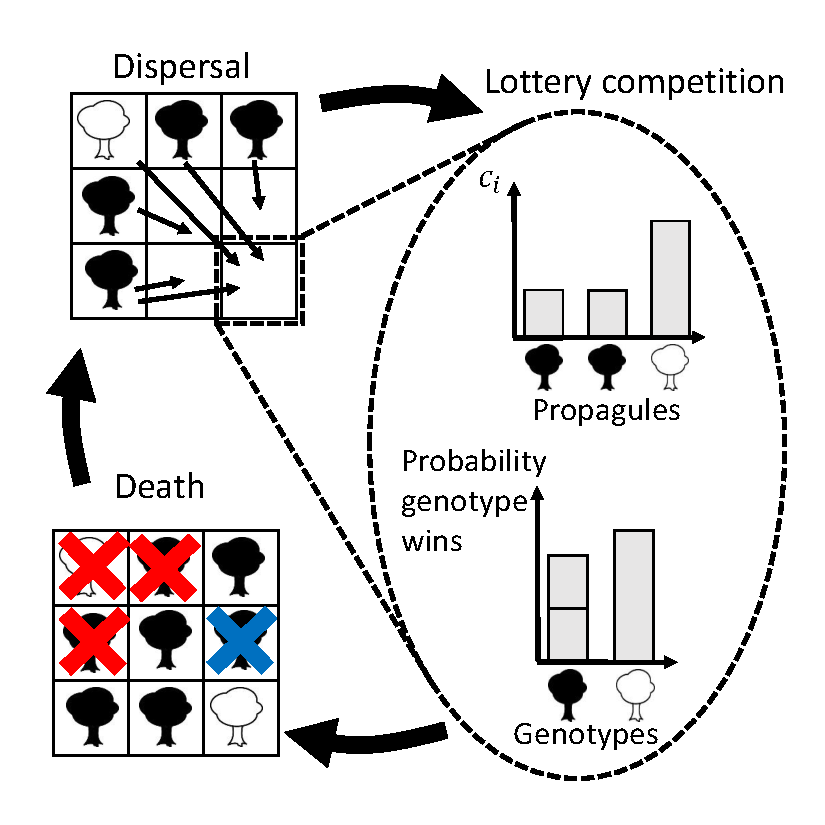
\includegraphics[scale=0.8]{lottery.pdf}
\caption{\label{fig:lottery} Each iteration of our model has three elements. First, propagules are produced by adults and dispersed at random (only propagules landing on unoccupied territories are shown). Some territories may receive zero propagules. Lottery competition then occurs in each unoccupied territory that receives a propagule (only illustrated in one territory). Each type has a probability proportional to $c_i x_i$ of securing a given territory, where $c_i$ measures competitive ability and $x_i$ is the number of propagules that disperse there. In the illustrated territory, the black type disperses more propagules but is a poorer competitor. Territories are then made available by deaths among those adults present at the start of the iteration (red crosses).}
\end{figure}

Each iteration, adults produce new offspring (``propagules''), $m_i$ of which disperse to unoccupied territories. We assume that adults cannot be ousted from their territories, so that $m_i$ only includes propagules landing on unoccupied territories. Propagules disperse at random over the unoccupied territories, regardless of distance from their parents, and independently of each other. There is no interaction between propagules (e.g. avoidance of territories crowded with propagules). Loss of propagules during dispersal is subsumed into $m_i$. We assume that each adult produces a constant number $b_i$ of successfully dispersing propagules; the loss of propagules due to dispersal to occupied territories then implies $m_i=b_i(1-N/T)n_i$. Note that due to our assumption of uniform dispersal, the parameter $b_i$ can be thought of as a measure of ``colonization ability'', which combines fecundity and dispersal ability \citep{levins_71,tilman_94,bolker_99}. 

The number of individuals of the $i$'th type landing in any particular territory is denoted $x_i$. We assume that $x_i$ follows a Poisson distribution $p_i(x_i)=l_i^{x_i} e^{-l_i}/x_i!$, where $l_i=m_i/U$ is the mean territorial propagule density. This approximation becomes exact when the $n_i$ are large enough that drift in $n_i$ can be ignored (Appendix A).

When multiple propagules land on the same territory, the victor is determined by lottery competition: type $i$ wins a territory with probability $c_i x_i/\sum_j c_j x_j$, where $c_i$ is a constant representing relative competitive ability (Fig. \ref{fig:lottery}). We expect that a fraction $p_1(x_1)\ldots p_G(x_G)$ of the $U$ unoccupied territories will have the propagule composition $x_1,\ldots,x_G$. Type $i$ is expected to win $c_i x_i/\sum_j c_j x_j$ of these. Ignoring fluctuations about these two expectations (due to our no-drift, large $T$, large $n_i$ approximation), type $i$'s territorial acquisition is given by
\begin{equation}
\Delta_+ n_i=U\sum_{x_1,\ldots,x_G} \frac{c_i x_i}{\sum_j c_j x_j} p_1(x_1)\ldots p_G(x_G) \label{eq:growthsumuncoupled}
\end{equation}
in our extended lottery model, where the sum only includes territories with at least one propagule present.

Finally, we assume that mortality only occurs in adults (setting aside the juvenile deaths implicit in territorial contest), and at a constant, type-specific per-capita rate $0\leq d_i\leq 1$, so that the overall change in type abundances is
\begin{equation}
\Delta n_i=\Delta_+ n_i-d_i n_i. \label{eq:delttot}
\end{equation}

\subsection*{Connection to the Wright-Fisher and classic lottery models}

In the classic lottery model \citep{chesson_1981}, unoccupied territories are assumed to be saturated with propagules from every type $l_i\gg 1$. From the law of large numbers, the composition of propagules in each territory will then not deviate appreciably from the mean composition $l_1,l_2,\ldots,l_G$ ($G$ is the number of types present), and so the probability that type $i$ wins any particular unoccupied territory is approximately $c_i l_i/\sum_j c_j l_j$. Then the numbers of territories won by each type $\Delta_+ n_1,\Delta_+ n_2,\ldots,\Delta_+ n_G$ follow a multinomial distribution with $U$ trials and success probabilities $\frac{c_1 l_1}{\sum_j c_j l_j},\frac{c_2 l_2}{\sum_j c_j l_j},\ldots,\frac{c_G l_G}{\sum_j c_j l_j}$, respectively. Type $i$ is expected to win $c_i l_i/\sum_j c_j l_j$ of the $U$ available territories, and deviations from this expected outcome are small (since $T$ is large by assumption), giving 
\begin{equation}
\Delta_+ n_i=\frac{c_i l_i}{\sum_j c_j l_j}U=\frac{c_i l_i}{\overline{c}L}U, \label{eq:lottery}
\end{equation}
where $\overline{c}=\sum_j c_j m_j/M$ is the mean propagule competitive ability for a randomly selected propagule, $L=M/U$ is the total propagule density and $M=\sum_j m_j$ is the total number of propagules. In section ``Analytical approximation of the density-dependent lottery'', we derive a generalization of Eq.~\eqref{eq:lottery} that accommodates arbitrary propagule densities $l_i$.
 
There is a close connection between the classic lottery model and the Wright-Fisher model of genetic drift \citep{svardal_2015}. In the Wright-Fisher model, type abundances are sampled each generation from a multinomial distribution with success probabilities $w_i n_i/\sum_j w_j n_j$, where $w$ is relative fitness and the $n_i$ are  type abundances in the preceding generation. Population size $N$ remains constant. This is equivalent to the classic lottery model with non-overlapping generations ($d_i=1$ for all $i$) and relative fitness given by $w_i=b_i c_i$ i.e. a product of fecundity and viability \citep[pp. 185]{crow_1970}. Thus, the classic lottery model is essentially the Wright-Fisher model extended to allow overlapping generations, but ignoring drift. This means that our extension of the classic lottery model to arbitrary densities represents a density-dependent generalization of the Wright-Fisher model (we also do not consider drift here).

\section*{Results}

\subsection*{Analytical approximation of the density-dependent lottery}

Eq. \eqref{eq:growthsumuncoupled} involves an expectation over the time-dependent dispersal distributions $p_i$, and is thus too complicated to give intuition about the dynamics of density-dependent lottery competition. We now evaluate this expectation. 

Similarly to the high-$l_i$ approximation of the classic lottery model, we replace the $x_i$ with appropriate mean values, although we cannot simply replace $x_i$ with $l_i$ as in Eq.~\eqref{eq:lottery}. The classic lottery model breaks down for types with low propagule density ($l_i\ll 1$) because territorial acquisition is then not correctly represented by a lottery in each territory with the mean propagule density. For a type with low propagule density $l_i\ll 1$, we have $x_i=1$ in the territories where its propagules land, and so its growth comes entirely from territories which deviate appreciably from $l_i$. To account for this, we separate Eq. \eqref{eq:growthsumuncoupled} into $x_i=1$ and $x_i>1$ parts. Our more general approximation only requires that there are no large discrepancies in competitive ability (i.e. we do not have $c_i/c_j\gg 1$ for any two types). We obtain (details in Appendix B)
\begin{equation}
\Delta_+ n_i\approx \left[e^{-L}+(R_i+A_i)\frac{c_i}{\overline{c}}\right]l_i U, \label{eq:master}
\end{equation}
where
\begin{equation}
R_i=\frac{\overline{c}e^{-l_i}(1-e^{-(L-l_i)})}{c_i +\frac{\overline{c}L- c_il_i}{L-l_i}\frac{L-1+e^{-L}}{1-(1+L)e^{-L}}},\nonumber \label{eq:Dr}
\end{equation}
and
\begin{equation}
A_i=\frac{\overline{c}(1-e^{-l_i})}{\frac{1-e^{-l_i}}{1-(1+l_i)e^{-l_i}}c_il_i+\frac{\overline{c}L- c_il_i}{L-l_i}\left(L\frac{1-e^{-L}}{1-(1+L)e^{-L}}-l_i\frac{1-e^{-l_i}}{1-(1+l_i)e^{-l_i}}\right)}. \nonumber \label{eq:Da}
\end{equation}

Comparing Eq. \eqref{eq:master} to Eq. \eqref{eq:lottery}, the classic lottery per-propagule success rate $c_i/\overline{c}L$ has been replaced by three separate terms. The first, $e^{-L}$, accounts for propagules which land alone on unoccupied territories; these territories are won without contest. The second, $R_i c_i/\overline{c}$, represents competitive victories when the $i$ type is a rare invader in a high density population (i.e. it determines invasion fitness \citep{metz_1992}). The third term, $A_i c_i/\overline{c}$, represents competitive victories when the $i$ type is abundant. The relative importance of these three terms varies with both the overall propagule density $L$ and the relative propagule frequencies $l_i/L$. If $l_i\gg 1$ for all types, we recover the classic lottery model (only the $A_ic_i/\overline{c}$ term remains, and $A_i\rightarrow 1/L$). 

Fig.~\ref{fig:simcomp} shows that Eq. \eqref{eq:master} and its components closely approximate simulations of the density-dependent lottery model over a wide range of propagule densities. Two types are present, one of which is at low frequency. The growth of the low-frequency type relies crucially on the low-density competition term $R_i c_i/\overline{c}$. On the other hand, $R_i c_i/\overline{c}$ is negligible for the high-frequency type, which depends instead on high density territorial victories. Fig.~\ref{fig:simcomp} also shows the breakdown of the classic lottery model at low propagule densities.

\begin{figure}
\centering
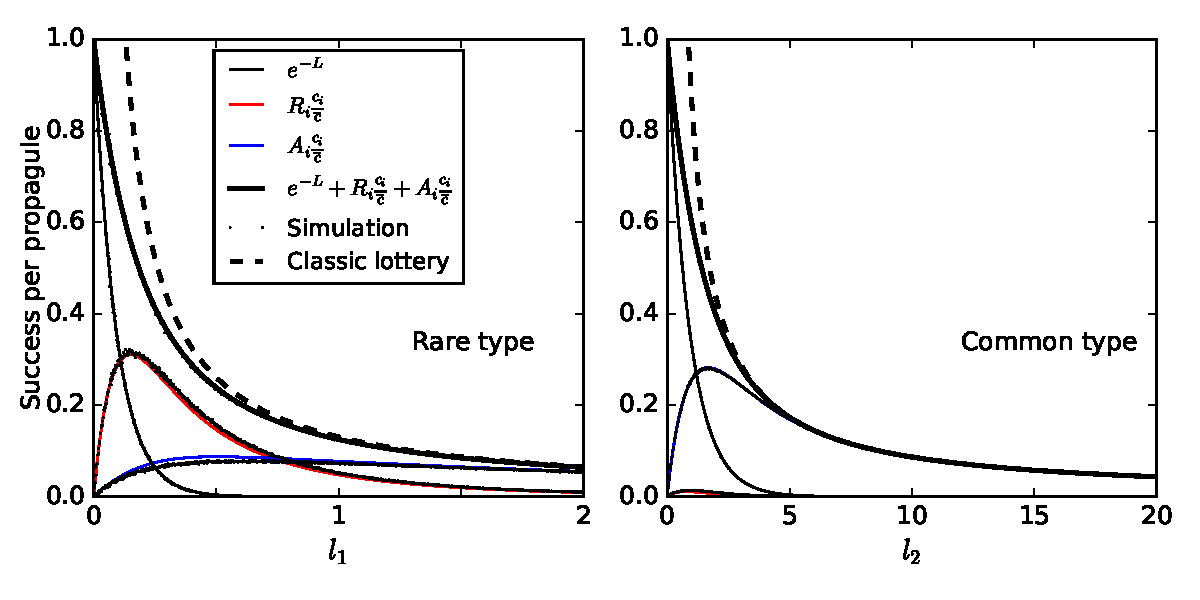
\includegraphics[scale=0.8]{simulationcomparison.pdf}
\caption{\label{fig:simcomp} Comparison of the analytical approximation Eq. \eqref{eq:master} with simulations. Per-propagule success probability $\Delta_+ n_i/l_i U$ from the classic lottery model, individual-based simulations of random dispersal and lottery competition, and Eq. \eqref{eq:master} and its three components. Two types are present, a rare type with $c_1=1.5$, and a common type with $c_2=1$. Simulation points are almost invisible in for the common type due to near exact agreement with Eq. \eqref{eq:master}. Dashed lines in show the breakdown of the classic lottery model. Parameters: $m_1=10^4$ and $m_2=9\times 10^4$ and $U$ varies between $5\times 10^3$ and $10^6$.} 
\end{figure}

Eq.~\eqref{eq:master} takes a much simpler form if all types are competitively equivalent ($c_i=c$),
\begin{equation}
\Delta_+ n_i = \frac{l_i}{L}(1-e^{-L})U. \label{eq:masterequalc}
\end{equation}
Here $1-e^{-L}$ is the fraction of territories that receive at least one propagule under Poisson dispersal, $(1-e^{-L})U$ is the total number of territories gained, and type $i$ receives $l_i/L$ of these. Total population density thus grows according to
\begin{equation}
\Delta N=(1-e^{-L})U-\sum_i d_i n_i \label{eq:Nmaster}
\end{equation}

\subsection*{$K$-selection versus relative fitness}

We now compare the density-dependent lottery model from the previous section with MacArthur's analysis of selection in crowded environments \citep{macarthur_1967}. MacArthur considers a population with two types that have densities $n_1$ and $n_2$ subject to density-dependent growth described by
\begin{equation}
\frac{d n_1}{d t}=f_1(n_1,n_2)\qquad\frac{d n_2}{d t}=f_2(n_1,n_2). \label{eq:macgeneral}
\end{equation}
The environment is assumed to remain constant apart from the type densities. The functions $f_1$ and $f_2$ must decline to zero if $n_1$ or $n_2$ are sufficiently large, because no population has unlimited resources. This defines the nullclines $f_1(n_1,n_2)=0$ and $f_2(n_1,n_2)=0$ in $(n_1,n_2)$ space. The outcome of selection is then determined by the relationship between these nullclines. Specifically, a type will be excluded if its nullcline is completely contained in the region bounded by the other type's nullcline. In other words, for a type to have the possibility of persisting, it must be able to keep growing to higher densities than the other type can tolerate in some region of $(n_1,n_2)$ space (Fig.~\ref{fig:Ksel}a).

To formalize the relationship between nullclines, MacArthur used the symbol ``$K$'' to label the four intersection points of the nullclines with the $n_1$ and $n_2$ axes, specifically $f_1(K_{11},0)=0$, $f_1(0,K_{12})=0$, $f_2(0,K_{22})=0$ and $f_2(K_{21},0)=0$. These $K$ values determine whether a region of higher-density growth exists for each type, provided that the nullclines are close to being straight lines. Note that only $K_{11}$ and $K_{22}$ are saturation densities akin to the $K$ parameter in the logistic model; following widespread convention, we will refer to selection on these saturation densities as ``$K$-selection'' (Fig.~\ref{fig:Ksel}a). The other intersection points, $K_{12}$ and $K_{21}$, are related to competition between types. For instance, in the Lotka-Volterra competition model we have
\begin{align}
f_1(n_1,n_2) = r_1(1-\alpha_{11}n_1-\alpha_{12}n_2)n_1\nonumber\\
f_2(n_1,n_2) = r_2(1-\alpha_{22}n_1-\alpha_{21}n_2)n_2\label{eq:LV}
\end{align}
where $\alpha_{11}=1/K_{11}$ and $\alpha_{22}=1/K_{22}$ measure competitive effects within types, while $\alpha_{12}=1/K_{12}$ and $\alpha_{21}=1/K_{21}$ measure competitive effects between types (Fig.~\ref{fig:LVvslottery}a). 

Thus, when MacArthur concludes that  ``fitness is $K$'' in crowded populations \citep[pp. 149]{macarthur_1967}, the meaning is that selection either favors the ability to keep growing at ever higher densities (moving a type's own nullcline outwards), or the ability to suppress the growth of competitors at lower densities (moving the nullcline of competitors inwards) \citep{gill_1974}. This general idea applies even if the nullclines are nonlinear to such an extent that the ``$K$'' values themselves do not give much information about the regions of high-density growth.

\begin{figure}
\centering
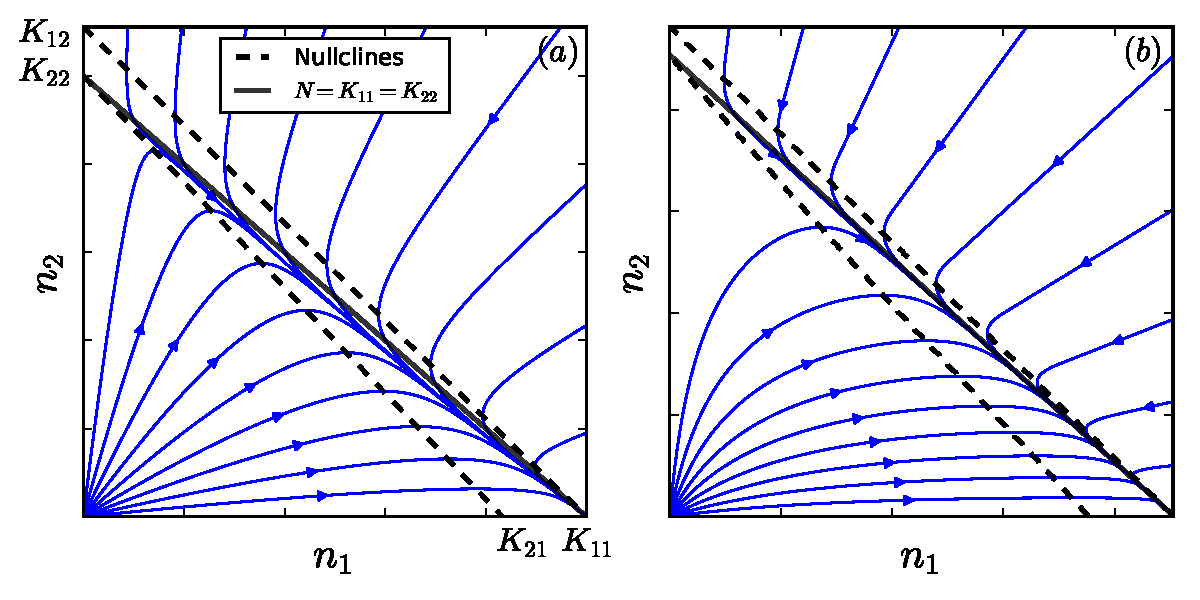
\includegraphics[scale=0.8]{LVvslottery.pdf}
\caption{\label{fig:LVvslottery} Selection between types with identical saturation density but different inter-type competitive ability. (a) Lotka-Volterra competition (Eq.~\ref{eq:LV}) with $r_1=r_2=1$, $\alpha_{11}=\alpha_{22}=1$, $\alpha_{12}=0.9$ and $\alpha_{21}=1.2$. Trajectories do not follow the line $N=K_{11}=K_{22}$. (b) Lottery competition (Eq.~\ref{eq:master}) with $b_1=b_2=5$, $d_1=d_2=0.1$ and $c_1/c_2=5$. Trajectories converge on the line $N=K_{11}=K_{22}$.}
\end{figure}

It is obvious from Eq.~\eqref{eq:LV} that selection can favor a superior competitor in a crowded population even if its saturation density is the same as, or lower than that of the other types present. However, note that the Lotka-Volterra model still closely couples selection to population density \citep{smouse_1976}. Fig.~\ref{fig:LVvslottery}a shows Lotka-Volterra selection between two types with the same saturation density ($\alpha_{11}=\alpha_{22}$, $\alpha_{21}>\alpha_{12}$). Even though the initial and final densities of a sweep are the same, density is not constant over a sweep. Only a highly restricted subset of $r$ and $\alpha$ values will keep $N$ constant over a selective sweep (further details in Appendix C). Intuitively, for one type to exclude another with the same saturation density, competitive suppression of growth between types must be stronger than competitive suppression of growth within types, causing a dip in $N$ over the sweep. 

By contrast, if one type in our density-dependent lottery model has a $c$ advantage but the types are otherwise identical (so that each type has the same saturation density), the density trajectories converge on the line of constant density equal to the saturation density (Fig.~\ref{fig:LVvslottery}b). Selection then occurs purely along this line, similarly to Fig.~\ref{fig:Ksel}b. This occurs because $c$ does not directly affect $N$: it only affects the relative likelihood for each type to win a contested territory, not whether a territory is contested in the first place (this can be seen formally in Eq.~\eqref{eq:Nmaster}). In other words, once the population reaches demographic equilibrium, it behaves indistinguishably from a constant-$N$ relative fitness model. While quite different from classical growth models like the Lotka-Volterra, this is all perfectly consistent with MacArthur's general argument. 

\subsection*{Density-dependence and the strength of selection}

We are now in a position to analyze the validity of Eq.~\eqref{eq:canonical} more explicitly. In the previous section we showed that selection and the regulation of population density can be completely independent of each other even if population growth is density-regulated, and moreover that MacArthur's general argument \citep{macarthur_1967} never precluded this possibility. Nevertheless, selection and density regulation \textit{are} intimately connected in widely used models of population growth. To understand why this poses a problem for Eq.~\eqref{eq:canonical}, consider the simple birth-death model \cite[pp. 20]{kostitzin_1939} 
\begin{equation}
\frac{d n_i}{dt}=(b_i -\delta_iN) n_i \label{eq:simplebirthdeath}
\end{equation}
where $\delta_i$ is the per-capita increase in type $i$'s mortality rate due to crowding (for simplicity, there are no deaths when uncrowded). Then, starting from a monomorphic population, the frequency of an adaptive $\delta$-variant $\delta_i\rightarrow \delta_i(1-\epsilon)$ obeys 
\begin{equation}
\frac{d p_i}{dt}=\epsilon \delta_i N p_i(1-p_i). \label{eq:Ndependentsweep}
\end{equation}
The selection coefficient $s=\epsilon \delta_i N$ thus depends on density (compare with Model III in \cite{kimura1969natural}). On the other hand, the frequency of an adaptive $b$-variant $b_i\rightarrow b_i(1+\epsilon)$ will exactly obey Eq.~\eqref{eq:canonical} with $s=\epsilon b_i$, independent of density.

In practice the density dependence in Eq.~\eqref{eq:Ndependentsweep} only matters if $N$ changes substantially during a sweep. This can easily occur if a population is far from demographic equilibrium (we return to this scenario in the Discussion). However, even if $N$ has reached equilibrium, it will change substantially over a $\delta$-sweep if selection on $\delta$ is sufficiently strong. To quantify this effect, we need to account for how much $N$ changes as a result of a $\delta$-sweep beginning and ending in equilibrium \citep{kimura1969natural}; from Eq.~\eqref{eq:simplebirthdeath} we have an increase from $N_{\rm initial}=b_i/\delta_i$ to $N_{\rm final}=b_i/\delta_i(1-\epsilon)=N_{\rm initial}/(1-\epsilon)$. The corresponding selection coefficient increases from $s_{\rm initial}= \epsilon b_i$ to $s_{\rm final}=s_{\rm initial}/(1-\epsilon)$. Consequently, substantial deviations from Eq.~\eqref{eq:canonical} occur with proportional changes to $\delta$ of order $\epsilon=0.1$ and upwards (Fig.~\ref{fig:strengthofselection}). 

\begin{figure}
\centering
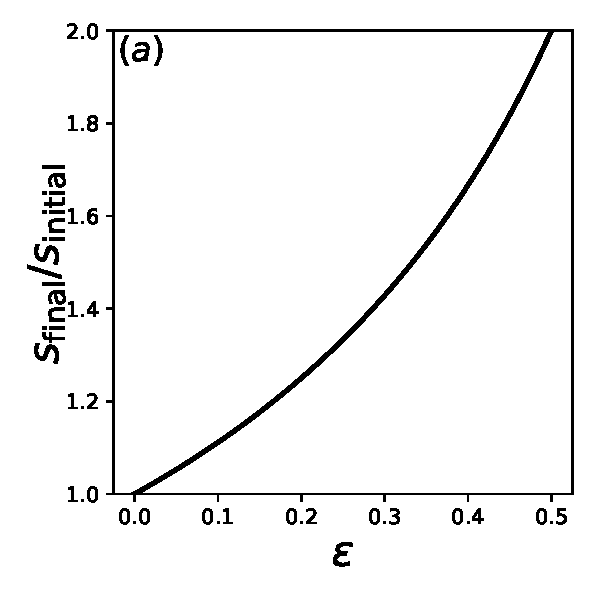
\includegraphics[scale=0.8]{strengthofselection.pdf}
\caption{\label{fig:strengthofselection} Proportional change in the selection coefficient over a ``$K$-selection''-type sweep for a type that experiences proportionally $1-\epsilon$ fewer deaths induced by crowding. The population is in demographic equilibrium at the start of the sweep.}
\end{figure}

Let us now contrast the simple linearly density-dependent model Eq.~\eqref{eq:simplebirthdeath} with our density-dependent lottery. Selection on $c$ is clearly density-dependent, but since selection on $c$ does not affect density (section ``$K$-selection versus relative fitness''), selection on $c$ does not introduce density-dependence in Eq.~\eqref{eq:canonical}.  

Turning to selection on $b$ and $d$, recall that $m_i=b_i n_i U/T$, and so $L=M/U=\overline{b}N/T$ where $\overline{b}$ is the population mean $b$. Thus, from Eq.~\eqref{eq:masterequalc} we have
\begin{equation}
\Delta n_i = \left(\frac{b_i}{\overline{b}}\frac{1-e^{-\overline{b}N/T}}{N}(T-N)-d_i\right)n_i. \label{eq:bdensitydependence}
\end{equation}
The mortality $d$ is akin to the birth rate in Eq.~\eqref{eq:simplebirthdeath}, and so, while $d$ does affect density, selection on $d$ is density independent, and so $d$ sweeps also follow the canonical relative fitness model exactly.

At first glance $b$ in Eq.~\eqref{eq:bdensitydependence} appears to be analogous to the $\delta$ in Eq.~\eqref{eq:simplebirthdeath} because it regulates density and is multiplied by the density-dependent term $f(\overline{b},N)=\frac{1-e^{-\overline{b}N/T}}{N}(T-N)$. This term declines from $\overline{b}$ at low density to zero at high density and as a result, selection on $b$ is density-dependent. In words: the selective advantage from having greater $b$ depends on the number of territories being contested; if almost all are occupied, then there is little advantage to having a greater $b$.

Nevertheless, the behavior of equilibrium-to-equilibrium $b$-sweeps are qualitatively different from the $\delta$ sweeps above. The reason is that $b$ does not regulate density via the $b_i$ term in front of $f(\overline{b},N)$, which is divided by $\overline{b}$ and thus actually reflects relative lottery contests. The density regulating effect of $b$ actually appears in the fraction of contested territories $1-e^{-\overline{b}N/T}$. This reflects the fact that $b$ sweeps can only increase density by causing more unoccupied territories to receive propagules. The net effect on $f(\overline{b},N)$ is precisely zero. To see this, note that in a single-type equilibrium we have $b_i/\overline{b}=1$ and so, setting Eq.~\eqref{eq:bdensitydependence} to zero, we $f(\overline{b},N)=d_i$ exactly at the beginning and end of a pure $b$ sweep, even though the density $N$ increases. Strictly speaking there is some deviation in $f(N)$ from $d_i$ during the sweep, but this deviation is an order of magnitude smaller than for a $\delta$ sweep (the deviation due to a sweep with proportional effect $b_i\rightarrow b_i(1+\epsilon)$ is only of order $\epsilon^2$, whereas the analogous effect in Fig.~\ref{fig:strengthofselection} is of order $\epsilon$; see Appendix D for details). Since selection must already be quite strong for a $\delta$ sweep to threaten Eq.~\eqref{eq:canonical}, we can safely conclude that $b$ sweeps obey Eq.~\eqref{eq:canonical} to a very close approximation.

To summarize: (i) $c$-selection is density-dependent, but $c$ does not affect density (ii) $d$-selection is density-independent but $d$ affects density (iii) $b$ affects density and is subject to density-dependent selection. And yet pure $b$, $c$ and $d$ sweeps starting and ending at equilibrium all obey the canonical selection equation exactly (almost exactly for $b$).


\section*{Discussion}

It is widely recognized that the relative fitness description of selection is poorly integrated with the ecological literature on population growth \citep{mallet_2012}. This is not simply a lack of ecological realism on the part of relative fitness models. Rather, in many population growth models, only one life-history stage is represented, and the competitive effects resulting from crowding appear as a reduction in absolute fitness that only depends on the type densities at this life-history stage (e.g. the $n_i^2$ and $n_in_j$ terms in the Lotka Volterra equation). However, many species have a ``reproductive excess'' of juveniles that are considerably more fragile than their adult counterparts \citep{chesson_1983,turner1968population,kimura1969natural,nei1971fertility}. As a result, competition and the selection it induces can be concentrated at the juvenile phase, where a large reproductive excess allows for most juveniles to be competitively eliminated. In our lottery model, this excess appears when the number of propagules is greater than the number of available territories. Then only $\approx 1/L$ of the juveniles contesting available territories survive to adulthood. Note that unlike the role of adult density $n_i$ in single-life-stage models, it is the propagule densities $l_i$ that represent the crowding that drives competition. In general, reproductive excesses will tend to produce strictly-relative lottery-type contests in which fitter types can grow at the expense of others by preferentially filling the available adult ``slots''. The number of slots can remain fixed or change independently of selection at the juvenile stage. By ignoring reproductive excesses, single life-stage models are biased to have total population density be sensitive to ongoing selection, artificially invalidating Eq.~\eqref{eq:canonical}. In this respect, the Wright-Fisher model and similar ``viability selection'' models actually capture an important ecological process.

We now turn to the breakdown of Eq.~\eqref{eq:canonical}. We first discuss the problem shown in Fig.~\ref{fig:strengthofselection}, which occurs when strong selection changes (adult) population density and is also density-dependent. In our lottery model, this can only occur if and only if types differ in $c$ as well as $b$ or $d$. Why does our model need joint trait variation when the classical density-dependent selection literature is built on traits that behave like the $\delta$ in Eq.~\eqref{eq:canonical} \citep{christiansen_2004}? To briefly review: Based on a diploid, bi-allelic variant of the logistic model, the $r$/$K$ scheme posited a dichotomy between $r$-selection (uncrowded) and $K$-selection (crowded), with the latter taken to mean selection for greater saturation density \citep{gill_1974}. A more general Lotka-Volterra model introduces the inter-type $\alpha_{ij}$ competition coefficients, with selection on these termed ``$\alpha$-selection'' \citep{gill_1974,joshi_2001}. Thus we are left with $r$-selection (uncrowded) versus $K$- or $\alpha$-selection (crowded). The latter two forms of selection in crowded populations behave like selection on $\delta$ in that they are both density-dependent and cause density to change over a sweep (although $N$ only dips temporarily during an $\alpha$-sweep). 

By contrast, the density-dependent ($c$) and density-determining traits ($b$ and $d$) in our lottery model are independent. This trait separation highlights the two distinct directions in which density and selection interact: selection may depend on density, and density may depend on selection \citep{prout_1980}. The combination is needed to pose a threat to Eq.~\eqref{eq:canonical} (recall that we are still assuming $N$ is not far from equilibrium). In this respect the simple linear models that have become standard in discussions of density-dependent selection \citep{roughgarden_1979,christiansen_2004,mallet_2012} actually represent a complicated form of the density-selection interaction that confounds a key underlying issue. 

Note that while this is a conceptual reason to be wary of the classical density-dependent selection models, it is not clear how we should expect the trait variation in nature to align. For instance, should we expect mutations to generally affect $b$, $c$ and $d$ independently of each other, or pleiotropically such that $\delta$-like selection is prevalent? In the case of well-mixed indirect exploitation competition for consumable resources, the $R^*$ rule  suggests that $\delta$-like selection will be prevalent. However, for many populations consumable resources are not well-mixed. Spatial localization of consumable resources (e.g. due to restricted movement of  nutrients through soils) will tend to create a territorial situation similar to the lottery model, where resource competition only occurs locally and both it any interference competition are subsumed into the competitive ability $c$, which does not affect $N$. 

Relative fitness models truly break down when $N$ is far from equilibrium and selection is density-dependent. For example, wild \textit{Drosophila} experience huge seasonal boom-bust cycles in population density coupled to strong selection that drives large swings in allele frequency \citep{bergland_14}. In this case there is no choice but to abandon relative fitness, and our model provides one potentially suitable option. Whether or not our density-dependent lottery model is a good description of \textit{Drosophila} ecology, the close connection between our model and Wright-Fisher is useful, because drift in our model should behave broadly similarly. Thus, our model it should provide a useful starting point for analyzing evolution in this and other from-from-equilibrium situations.

\section*{Acknowledgments}

We thank Peter Chesson and Joachim Hermisson for many constructive comments on an earlier and quite different version of this manuscript. This work was financially supported by the National Science Foundation (DEB-1348262) and the John Templeton Foundation (60814).

\bibliographystyle{plainnat}
\bibliography{reference} 

\section*{Appendix A: Poisson approximation}

For simplicity of presentation, we have assumed a Poisson distribution for the $x_i$ as our model of dispersal. Strictly speaking, the total number of $i$ propagules $\sum x_i$ (summed over unoccupied territories) is then no longer a constant $m_i$, but fluctuates between generations for a given mean $m_i$, which is more biologically realistic. Nevertheless, since we do not consider the random fluctuations in type abundances here, and for ease of comparison with the classic lottery model, we ignore the fluctuations in $m_i$. Instead we focus, on Poisson fluctuations in propagule composition in each territory. 

In the exact model of random dispersal, the counts of a type's propagules across unnocupied territories follows a multinomial distribution with dimension $U$, total number of trials equal to $m_i$, and equal probabilities $1/U$ for a propagule to land in a given territory. Thus, the $x_i$ in different territories are not independent random variables. However, for sufficiently large $U$ and $m_i$, this multinomial distribution for the $x_i$ across territories is closely approximated by a product of independent Poisson distributions for each territory, each with rate parameter $l_i$ \citep[Theorem 1]{arenbaev_1977}. Since we are ignoring finite population size effects, we effectively have $T\rightarrow \infty$, in which case $U$ can be only be small enough to violate the Poisson approximation if there is vanishing population turnover, and then the dispersal distribution is irrelevant anyway. Likewise, in ignoring stochastic finite population size for the $n_i$, we have effectively already assumed that $m_i$ is large enough to justify the Poisson approximation (the error scales as $1/\sqrt{m_i}$; \citealt{arenbaev_1977}).

\section*{Appendix B: Derivation of growth equation}

We separate the right hand side of Eq.~\eqref{eq:growthsumuncoupled} into three components $\Delta_+ n_i = \Delta_u n_i+\Delta_r n_i+\Delta_a n_i$ which vary in relative magnitude depending on the propagule densities $l_i$. Following the notation in the main text, the Poisson distributions for the $x_i$ (or some subset of the $x_i$) will be denoted $p$, and we use $P$ as a general shorthand for the probability of particular outcomes.

\subsection*{Growth without competition}

The first component, $\Delta_u n_i$, accounts for territories where only one focal propagule is present $x_i=1$ and $x_j=0$ for $j\neq i$ ($u$ stands for ``uncontested''). The proportion of territories where this occurs is $l_i e^{-L}$, and so 
\begin{equation}
\Delta_u n_i=Ul_i e^{-L}=m_i e^{-L}.
\end{equation}

\subsection*{Competition when rare}

The second component, $\Delta_r n_i$, accounts for territories where a single focal propagule is present along with at least one non-focal propagule ($r$ stands for ``rare'') i.e. $x_i=1$ and $X_i\geq 1$ where $X_i=\sum_{j\neq i} x_j$ is the number of nonfocal propagules. The number of territories where this occurs is $Up_i(1)P(X_i\geq 1)=b_i n_i e^{-l_i}(1-e^{-(L-l_i)})$. Thus 
\begin{equation}
\Delta_r n_i = m_i e^{-l_i}(1-e^{-(L-l_i)})\left\langle  \frac{c_i}{c_i +\sum_{j\neq i} c_j x_j } \right\rangle_{\tilde{p}},  \label{eq:deltr}
\end{equation}
where $\langle \rangle_{\tilde{p}}$ denotes the expectation with respect to $\tilde{p}$, and $\tilde{p}$ is the probability distribution of nonfocal propagule abundances $x_j$ \textit{after} dispersal, in those territories where exactly one focal propagule, and at least one non-focal propagule, landed. 

Our ``mean field'' approximation is to replace $x_j$ with its mean in the last term in Eq.~\eqref{eq:deltr},
\begin{equation}
\left\langle\frac{c_i}{c_i +\sum_{j\neq i} c_j x_j}\right\rangle_{\tilde{p}}\approx \frac{c_i}{c_i +\sum_{j\neq i} c_j \langle x_j\rangle_{\tilde{p}}}.\label{eq:meanfieldr}
\end{equation}
Below we justify this replacement by arguing that the standard deviation $\sigma_{\tilde{p}}(\sum_{j\neq i} c_j x_j)$ (with respect to $\tilde{p}$), is much smaller than $\langle\sum_{j\neq i} c_j x_j\rangle_{\tilde{p}}$.

We first calculate $\langle x_j \rangle_{\tilde{p}}$. Let $X=\sum_j x_j$ denote the total number of propagules in a territory and ${\mathbf x_i}=(x_1,\ldots,x_{i-1},x_{i+1}\ldots,x_G)$ denote the vector of non-focal abundances, so that $p({\mathbf x_i})=p_1(x_1)\ldots p_{i-1}(x_{i-1})p_{i+1}(x_{i+1})\ldots p_G(x_G)$. Then, $\tilde{p}$ can be written as
\begin{align}
\tilde{p}({\mathbf x_i})&=p({\mathbf x_i}|X\geq 2,x_i=1)\nonumber\\
&=\frac{P({\mathbf x_i},X\geq 2|x_i=1)}{P(X\geq 2)}\nonumber\\
&=\frac{1}{1-(1+L)e^{-L}}\sum_{X=2}^{\infty} P(X) p({\mathbf x_i}|X_i=X-1),
\end{align}
and so
\begin{align}
\langle x_j \rangle_{\tilde{p}}&=\sum_{\mathbf x_i} \tilde{p}({\mathbf x_i})x_j\nonumber\\
&=\frac{1}{1-(1+L)e^{-L}}\sum_{X=2}^{\infty} P(X) \sum_{\mathbf x_i} p({\mathbf x_i}|X_i=X-1)x_j.
\label{eq:raremonster1}
\end{align}
The inner sum over ${\mathbf x_i}$ is the mean number of propagules of a given nonfocal type $j$ that will be found in a territory which received $X-1$ nonfocal propagules in total, which is equal to $\frac{l_j}{L-l_i}(X-1)$. Thus, 
\begin{align}
\langle x_j \rangle_{\tilde{p}}&=\frac{l_j}{1-(1+L)e^{-L}}\frac{1}{L-l_i}\sum_{k=2}^{\infty} P(X) (X-1)\nonumber\\
&=\frac{l_j}{1-(1+L)e^{-L}}\frac{L-1+e^{-L}}{L-l_i},
\label{eq:meanxjrare}
\end{align}
where the last line follows from $\sum_{X=2}^{\infty} P(X)(X-1)=\sum_{X=1}^{\infty} P(X)(X-1)=\sum_{X=1}^{\infty} P(X)X-\sum_{X=1}^{\infty}P(X)$.

The exact analysis of the fluctuations in $\sum_{j\neq i} c_j x_j$ is complicated because the $x_j$ are not independent with respect to $\tilde{p}$. These fluctuations are part of the ``drift'' in type abundances which we leave for future work. Here we use the following approximation to give some insight into the magnitude of these fluctuations and also the nature of the correlations between the $x_j$. We replace $\tilde{p}$ with $\tilde{q}$, defined as the ${\mathbf x_i}$ Poisson dispersal probabilities conditional on $X_i\geq1$ (which are independent). The distinction between $\tilde{p}$ with $\tilde{q}$ will be discussed further below. The $\tilde{q}$ approximation gives $\langle x_j \rangle_{\tilde{q}}=\langle x_j \rangle_p/C=l_j/C$, 
\begin{align}
\sigma_{\tilde{q}}^2(x_j)&=\langle x_j^2 \rangle_{\tilde{q}}-\langle x_j \rangle_{\tilde{q}}^2\nonumber\\
&=\frac{1}{C}\langle x_j^2 \rangle_p-\frac{l_j^2}{C^2}\nonumber \\
&=\frac{1}{C}(l_j^2 + l_j)-\frac{l_j^2}{C^2}\nonumber \\
&=\frac{l_j^2}{C}\left(1-\frac{1}{C}\right)+\frac{l_j}{C},\label{eq:varr}
\end{align}
and 
\begin{align}
\sigma_{\tilde{q}}(x_j,x_k)&=\langle x_j x_k \rangle_{\tilde{q}}-\langle x_j \rangle_{\tilde{q}}\langle x_k \rangle_{\tilde{q}}\nonumber\\
&=\frac{1}{C}\langle x_j x_k \rangle_p-\frac{l_jl_k}{C^2}\nonumber\\
&=\frac{l_j l_k}{C}\left(1-\frac{1}{C}\right),\label{eq:covr}
\end{align}
where $C=1-e^{-(L-l_i)}$ and $j\neq k$. 

The exact distribution $\tilde{p}$ assumes that exactly one of the  propagules present in a given site after dispersal belongs to the focal type, whereas $\tilde{q}$ assumes that there is a focal propagule present before non-focal dispersal commences. As a result, $\tilde{q}$ predicts that the mean propagule density is greater than $L$ (in sites with only one focal propagule is present) when the focal type is rare and the propagule density is high. This is erroneous, because the mean number of propagules in every site is $L$ by definition. Specifically, if $L-l_i \approx L\gg 1$, then the mean propagule density predicted by $\tilde{q}$ is approximately $L+1$. The discrepancy causes rare invaders to have an intrinsic rarity disadvantage (territorial contests under $\tilde{q}$ are more intense than they should be). In contrast, Eq. \eqref{eq:meanxjrare} correctly predicts that there are on average $\sum_{j\neq i}\langle x_j \rangle_{\tilde{p}}\approx L-1$ nonfocal propagules because $\tilde{p}$ accounts for potentially large negative covariances between the $x_j$ ``after dispersal''. By neglecting the latter covariences, $\tilde{q}$ overestimates the fluctuations in $\sum_{j\neq i} c_j x_j$; thus $\tilde{q}$ gives an upper bound on the fluctuations. The discrepancy between $\tilde{q}$ and $\tilde{p}$ will be largest when $L$ is of order $1$ or smaller, because then the propagule assumed to already be present under $\tilde{q}$ is comparable to, or greater than, the entire propgaule density. 

Decomposing the variance in $\sum_{j\neq i} c_j x_j$,
\begin{equation}
\sigma_{\tilde{q}}^2(\sum_{j\neq i} c_j x_j)=\sum_{j\neq i}\left[c_j^2\sigma_{\tilde{q}}^2(x_j)+2\sum_{k>j, k\neq i}c_j c_k\sigma_{\tilde{q}}(x_j,x_k)\right],\label{eq:vartotr}
\end{equation}
and using the fact that $\sigma_{\tilde{q}}(x_j,x_k)$ and the first term in Eq. \eqref{eq:varr} are negative because $C<1$, we obtain an upper bound on the relative fluctuations in $\sum_{j\neq i} c_j x_j$, 
\begin{equation}
\frac{\sigma(\sum_{j\neq i} c_j x_j)}{\langle\sum_{j\neq i} c_j x_j\rangle}=C^{1/2}\frac{\left(\sum_{j\neq i}c_j^2 l_j+(1-1/C)\left(\sum_{j\neq i}c_j l_j\right)^2 \right)^{1/2}}{\sum_{j\neq i}c_j l_j}<C^{1/2}\frac{\left(\sum_{j\neq i}c_j^2 l_j\right)^{1/2}}{\sum_{j\neq i}c_j l_j}. \label{eq:cvr}
\end{equation}

Suppose that the $c_j$ are all of similar magnitude (their ratios are of order one). Then Eq.~\eqref{eq:cvr} is $\ll 1$ for the case when $L-l_i \ll 1$ (due to the factor of $C^{1/2}$), and also for the case when at least some of the nonfocal propagule densities are large $l_j\gg 1$ (since it is then of order $1/\sqrt{L-l_i}$). The worst case scenario occurs when $L-l_i$ is of order one. Then Eq.~\eqref{eq:cvr} gives a relative error of approximately $50\%$, which from our earlier discussion we know to be a substantial overestimate when $L$ is of order $1$. Our numerical results (Fig. \ref{fig:simcomp}) confirm that the relative errors are indeed small.

However, the relative fluctuations in $\sum_{j\neq i} c_j x_j$ can be large if some of the $c_j$ are much larger than the others. Specifically, in the presence of a rare, extremely strong competitor ($c_j l_j\gg c_{j'} l_{j'}$ for all other nonfocal types $j'$, and $l_j\ll 1$), then the RHS of Eq. \eqref{eq:cvr} can be large and we cannot make the replacement Eq.~\eqref{eq:meanfieldr}. 

Substituting Eqs. \eqref{eq:meanfieldr} and \eqref{eq:meanxjrare} into Eq.~\eqref{eq:deltr}, we obtain
\begin{equation}
\Delta_r n_i\approx m_i R_i\frac{c_i}{\overline{c}}, \label{eq:deltrfinal}
\end{equation}
where $R_i$ is defined in Eq.~\eqref{eq:Dr}.

\subsection*{Competition when abundant}

The final contribution, $\Delta_a n_i$, accounts for territories where two or more focal propagules are present ($a$ stands for ``abundant"). Similarly to Eq.~\eqref{eq:deltr}, we have 
\begin{equation}
\Delta_a n_i=U(1-(1+l_i)e^{l_i})\left\langle \frac{c_i x_i}{\sum_j c_j x_j} \right\rangle_{\hat{p}}\label{eq:delta}
\end{equation}
where $\hat{p}$ is the probability distribution of both focal and nonfocal propagaule abundances \textit{after} dispersal in those territories where at least two focal propagules landed. 

Again, we argue that the relative fluctuations in $\sum c_j x_j$ are much smaller than $1$ (with respect to $\hat{p}$), so that,
\begin{equation}
\left\langle \frac{c_i x_i}{\sum_j c_j x_j} \right\rangle_{\hat{p}}\approx  \frac{c_i \langle x_i \rangle_{\hat{p}}}{\sum_j c_j \langle x_j\rangle_{\hat{p}}}.\label{eq:meanfielda}
\end{equation}
Following a similar procedure as for $\Delta_r n_i$, where the vector of propagule abundances is denoted ${\mathbf x}$, the mean focal type abundance is, 
\begin{align}
\langle x_i \rangle_{\hat{p}}&=\sum_{\mathbf x} x_i p(\mathbf x|x_i\geq 2)\nonumber \\
&=\sum_{x_i} x_i p(x_i|x_i\geq 2) \nonumber\\
&=\frac{1}{1-(1+l_i)e^{-l_i}}\sum_{x_i\geq 2} p(x_i)x_i\nonumber\\
&=l_i\frac{1-e^{-l_i}}{1-(1+l_i)e^{-l_i}}.
\end{align}
For nonfocal types $j\neq i$, we have
\begin{align}
\langle x_j \rangle_{\hat{p}}&=\sum_{\mathbf x} x_j p(\mathbf x|x_i\geq 2)\nonumber \\
&=\sum_{X}P(X|x_i\geq 2)\sum_{\mathbf x} x_j p({\mathbf x}|x_i\geq 2,X)\nonumber\\
&=\sum_{X}P(X|x_i\geq 2)\sum_{x_i} p(x_i|x_i\geq 2,X) \sum_{\mathbf x_i} x_j p(\mathbf x_i|X_i=X-x_i)\nonumber\\
&=\sum_{X}P(X|x_i\geq 2)\sum_{x_i}p(x_i|x_i\geq 2,X) \frac{l_j(X-x_i)}{L-l_i} \nonumber\\
&=\frac{l_j}{L-l_i}\left[\sum_{X}P(X|x_i\geq 2)X - \sum_{x_i}p(x_i|x_i\geq 2) x_i \right]\nonumber\\
&=\frac{l_j}{L-l_i}\left( L\frac{1-e^{-L}}{1-(1+L)e^{-L}}- l_i\frac{1-e^{-l_i}}{1-(1+l_i)e^{-l_i}}\right). 
\end{align}

To calculate the relative fluctuations in $\sum_{j\neq i} c_j x_j$, we use a similar approximation as for $\Delta_r n_i$: $\hat{p}$ is approximated by $\hat{q}$, defined as the ${\mathbf x}$ dispersal probabilities in a territory conditional on $x_i>2$ (that is, treating the $x_j$ as indepenent). All covariances between nonfocal types are now zero, so that $\sigma_{\hat{q}}^2(\sum c_j x_j)=\sum c_j^2 \sigma_{\hat{q}}^2(x_j)$, where $\sigma_{\hat{q}}^2(x_j)=l_j$ for $j\neq i$, and  
\begin{equation}
\sigma_{\hat{q}}^2(x_i)=\frac{l_i}{D}\left(l_i+1-e^{-l_i}-\frac{l_i}{D}\left(1-e^{-l_i}\right)^2\right),
\end{equation}
where $D= 1-(1+l_i)e^{-l_i}$, and 
\begin{equation}
\frac{\sigma_{\hat{q}}(\sum c_j x_j)}{\langle\sum c_j x_j\rangle} = \frac{\left(\sum_{j\neq i} c_j^2 l_j + c_i^2 \sigma_{\hat{q}}^2(x_i)\right)^{1/2}}{\sum_{j\neq i} c_j l_j + c_i l_i (1-e^{-l_i})/D} \label{eq:cva}.
\end{equation}

Similarly to Eq.~\eqref{eq:cvr}, the RHS of Eq. \eqref{eq:cva} is $\ll 1$ for the case that $L \ll 1$ (due to a factor of $D^{1/2}$), and also for the case when at least some of the propagule densities (focal or nonfocal) are large --- provided that $c_i$ and the $c_j$ are all of similar magnitude. Again, the worst case scenario occurs when $l_i$ and $L-l_i$ are of order $1$, in which case Eq. \eqref{eq:cva} is around $35\%$, which is again where the $\hat{q}$ approximation produces the biggest overestimate of the fluctuations in ${\mathbf x}$. Similarly to Eq.~\eqref{eq:cvr}, the RHS of \eqref{eq:cva} will not be $\ll 1$ in the presence of a rare, extremely strong competitor.  

Combining Eqs. \eqref{eq:delta} and \eqref{eq:meanfielda}, we obtain
\begin{equation}
\Delta_a n_i=m_i A_i \frac{c_i}{\overline{c}},
\end{equation}
where $A_i$ is defined in Eq.~\eqref{eq:Da}.

\section*{Appendix C: Total density in the Lotka-Volterra competition model}

Here we show that under the Lotka-Volterra model of competition, total density $N$ does not in general remain constant over a selective sweep in a crowded population even if the types have the same saturation density (for a related discussion on the density- and frequency-dependence of selection in the Lotka-Volterra model, see \citep{smouse_1976,mallet_2012}).

We assume equal effects of crowding within types $\alpha_{11}=\alpha_{22}=\alpha_{\rm intra}$ and $N=1/\alpha_{\rm intra}$ and check whether it is then possible for $\frac{dN}{dt}$ to be zero in the sweep ($n_1,n_2 \neq 0$). Substituting these conditions into Eq.~\eqref{eq:LV}, we obtain 
\begin{align}
\frac{d n_1}{dt} = r_1(\alpha_{11}-\alpha_{12})n_1n_2 \nonumber\\
\frac{d n_2}{dt} = r_2(\alpha_{22}-\alpha_{21})n_1n_2
\end{align}
Adding these together, $\frac{dN}{dt}$ can only be zero if 
\begin{equation}
r_1(\alpha_{\rm intra}-\alpha_{12})+r_2(\alpha_{\rm intra}-\alpha_{21})=0. \label{eq:constNcondition}
\end{equation}
To get some intuition for Eq.~\eqref{eq:constNcondition}, suppose that a mutant arises with improved competitive ability but identical intrinsic growth rate and saturation density ($r_1=r_2$ and $\alpha_{11}=\alpha_{22}$). This could represent a mutation to an interference competition trait, for example \citep{gill_1974}. Then, according the above condition, for $N$ to remain constant over the sweep, the mutant must find the wildtype more tolerable than itself by exactly the same amount that the wildtype finds the mutant less tolerable than itself. 

Even if we persuaded ourselves that this balance of inter-type interactions is plausible in some circumstances, when multiple types are present the requirement for constant $N$ becomes
\begin{equation}
\sum_{ij}r_i(\alpha_{\rm intra}-\alpha_{ij})p_ip_j=0,
\end{equation}
which depends on frequency and thus cannot be satisfied in general for constant inter-type coefficients $\alpha_{ij}$. We conclude that selection in the Lotka-Volterra competition model will generally involve non-constant $N$.

\section*{Appendix D: Density-dependence of $b$-selection}

In section ``Density-dependence and the strength of selection'' we argued that the density-dependent factor $f(\overline{b},N)$ is unchanged at the beginning and end points of an equilibrium-to-equilibrium $b$. Here we estimate the magnitude of the deviation in $f(\overline{b},N)$ during the sweep. 

For simplicity, we introduce the notation $D=N/T$ and assume that $D$ is small. We can thus make the approximation $1-e^{-\overline{b}D}\approx \overline{b}D$ and $f(\overline{b},N)\approx \overline{b}(1-D)$. We expect this to be a conservative approximate based on the worst case scenario, because $N$ is most sensitive to an increase in $b$ in this low-density linear regime. We first calculate the value of $f(\overline{b},N)$ at the halfway point in a sweep, where the halfway point is estimated with simple linear averages for $b$ and $N$. The sweep is driven by a $b$ variant with $b_j=b_i(1+\epsilon)$, and we denote the corresponding initial and final densities by $D_i$ and $D_j$ respectively, where we have $d_i=b_i(1-D_i)=b_j(1-D_j)$. We obtain
\begin{align}
f_{\rm{half}}=f(\frac{b_i+b_j}{2},\frac{N_i+N_j}{2})&=\frac{b_i+b_j}{2}\left(1-\frac{D_i+D_j}{2}\right) \nonumber \\
&=\frac{1}{4} (b_i+b_j)(2-D_i-D_j) \nonumber \\
&=\frac{1}{4} (2d_i+b_i(1-D_j)+b_j(1-N_i)).
\end{align}
Dividing by $d_i$, the proportional deviation in $f(N)$ at the midpoint of the sweep is
\begin{align}
\frac{f_{\rm{half}}}{d_i}&=\frac{1}{4}\left(2+\frac{b_i}{b_j}+\frac{b_j}{b_i}\right)\nonumber \\
&=\frac{1}{4}\left(2+\frac{1}{1+\epsilon}+1+\epsilon\right)\nonumber \\
&=1+\frac{1}{4}(\epsilon^2-\epsilon^3+\ldots),
\end{align}
where we have used the Taylor expansion $\frac{1}{1+\epsilon}=1-\epsilon+\epsilon^2-\epsilon^3+\ldots$. 

By contrast, for a $\delta$ sweep in Eq.~\eqref{eq:simplebirthdeath}, the density-dependent term $N$ increases by a factor of $\frac{1}{1-\epsilon}=1+\epsilon+\epsilon^2+\ldots$. Thus,  the deviations in $f(N)$ are an order of magnitude smaller than those shown in Fig.~\eqref{fig:strengthofselection}, and even proportional changes of order $\epsilon=0.1$ will cause a negligible deviation from the canonical selection equation.


\end{document}

